\documentclass[english,11pt]{beamer}

\DeclareMathOperator{\Cov}{Cov}
\DeclareMathOperator{\Var}{Var}
\DeclareMathOperator{\E}{\mathbb{E}}
\DeclareMathOperator{\Proba}{\mathbb{P}}

\newcommand{\Covb}[2]{\ensuremath{\Cov\!\left[#1,#2\right]}}
\newcommand{\Eb}[1]{\ensuremath{\E\!\left[#1\right]}}
\newcommand{\Pb}[1]{\ensuremath{\Proba\!\left[#1\right]}}
\newcommand{\Varb}[1]{\ensuremath{\Var\!\left[#1\right]}}

% norm
\newcommand{\norm}[1]{\| #1 \|}

\newcommand{\indep}{\rotatebox[origin=c]{90}{$\models$}}





\usepackage{mathptmx,amsmath,amssymb,graphicx,bibentry,bbm,babel,ragged2e}

\makeatletter

\newcommand{\noun}[1]{\textsc{#1}}
\newcommand{\jitem}[1]{\item \begin{justify} #1 \end{justify} \vfill{}}
\newcommand{\sframe}[2]{\frame{\frametitle{#1} #2}}

\newenvironment{centercolumns}{\begin{columns}[c]}{\end{columns}}
%\newenvironment{jitem}{\begin{justify}\begin{itemize}}{\end{itemize}\end{justify}}

\usetheme{Warsaw}
\setbeamertemplate{footline}[text line]{}
\setbeamertemplate{headline}{}
\setbeamercolor{structure}{fg=purple!50!blue, bg=purple!50!blue}

\setbeamersize{text margin left=15pt,text margin right=15pt}

\setbeamercovered{transparent}


\@ifundefined{showcaptionsetup}{}{%
 \PassOptionsToPackage{caption=false}{subfig}}
\usepackage{subfig}

\usepackage[utf8]{inputenc}
\usepackage[T1]{fontenc}

\usepackage{multirow}

\usepackage{mdframed}


\makeatother

\begin{document}



\title{Assemblée Générale SoDUCo}

\subtitle{Propositions pour le WP3}

\author{J.~Raimbault$^{1,2,3,4}$\\
\texttt{juste.raimbault@ign.fr}
}


\institute{$^{1}$LASTIG, Univ Gustave Eiffel, IGN-ENSG\\
$^{2}$CASA, UCL\\
$^{3}$UPS CNRS 3611 ISC-PIF\\
$^{4}$UMR CNRS 8504 G{\'e}ographie-cit{\'e}s
}


\date{25/01/2022}

\frame{\maketitle}







\sframe{D{\'e}finition de la co-évolution}{

\justify
 
  \textbf{Objets : } Villes et territoires (\textit{Théorie {\'E}volutive des Villes}) qui co-évoluent avec les réseaux de transport (\textit{Théorie Territoriale des Réseaux})
 
 \medskip


\textbf{Processus : }

\textit{Une définition de la co-évolution à trois niveaux : } 
\begin{enumerate}
	\item \textcolor{blue}{niveau des agents}
	\item \textcolor{green}{niveau des populations d'agents (niches)}
	\item \textcolor{red}{niveau global du système}
\end{enumerate}  


\medskip


\textbf{Entrées : }

\begin{enumerate}
	\item \textcolor{blue}{Entrée empirique (niveau microscopique)}
	\item \textcolor{green}{Entrée par la morphogenèse (niveau de la niche)}
	\item \textcolor{red}{Entrée par la théorie évolutive (niveau global)}
\end{enumerate}

\medskip

\tiny

Raimbault, Juste (2019). Modeling interactions between transportation networks and territories: a co-evolution approach. arXiv preprint arXiv:1902.04802.
 
 \nocite{raimbault2019modeling}
 
}



\sframe{Méthode de caractérisation de la co-évolution}{

\begin{center}
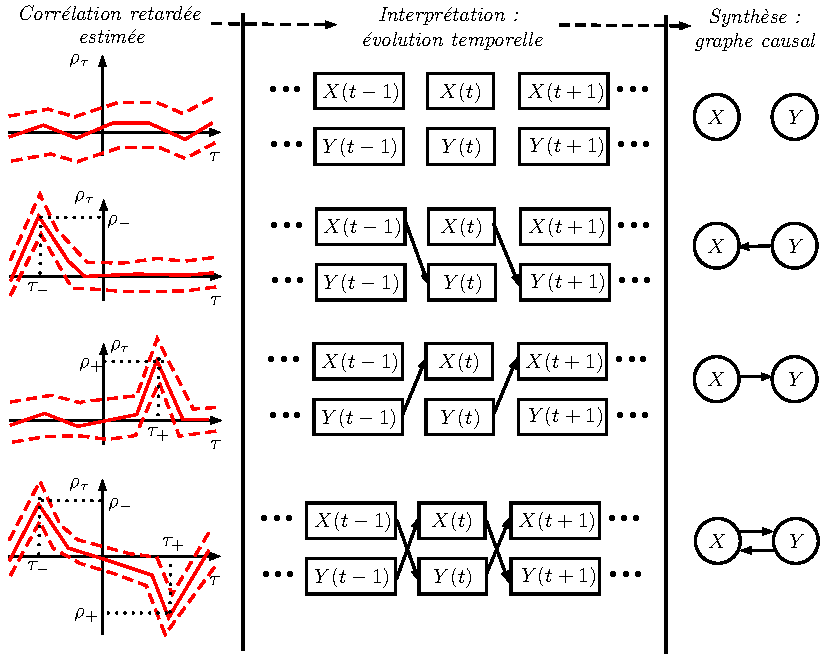
\includegraphics[width=0.8\linewidth]{figures/causality-method.pdf}
\end{center}

\tiny

Raimbault, J. (2017). Identification de causalités dans des données spatio-temporelles. In Spatial Analysis and GEOmatics 2017.

\nocite{raimbault2017identification}

}


\sframe{Modèles macroscopiques de co-évolution}{

\textit{Modèle d'interaction pour les systèmes de villes incluant l'évolution du réseau; production de multiples régimes de co-évolution et calibration pour la France (1830-2000).}

\medskip

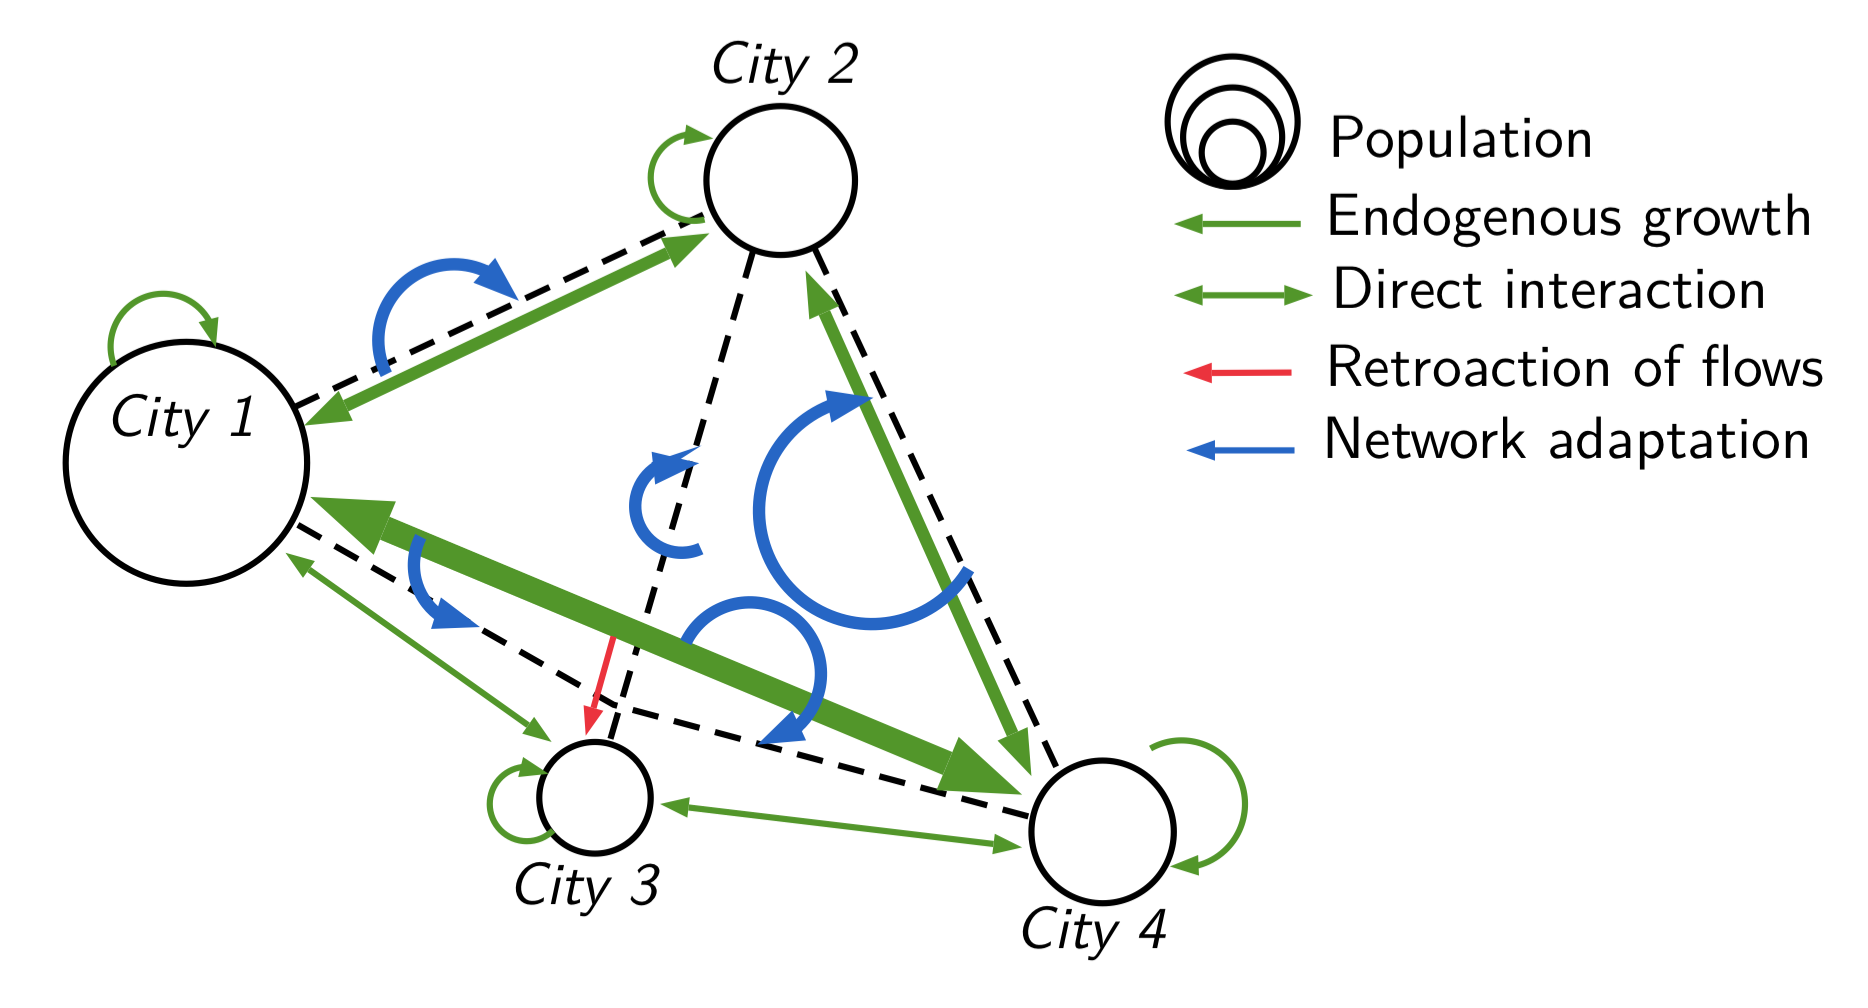
\includegraphics[width=0.6\textwidth]{figures/macrocoevol_en.png}
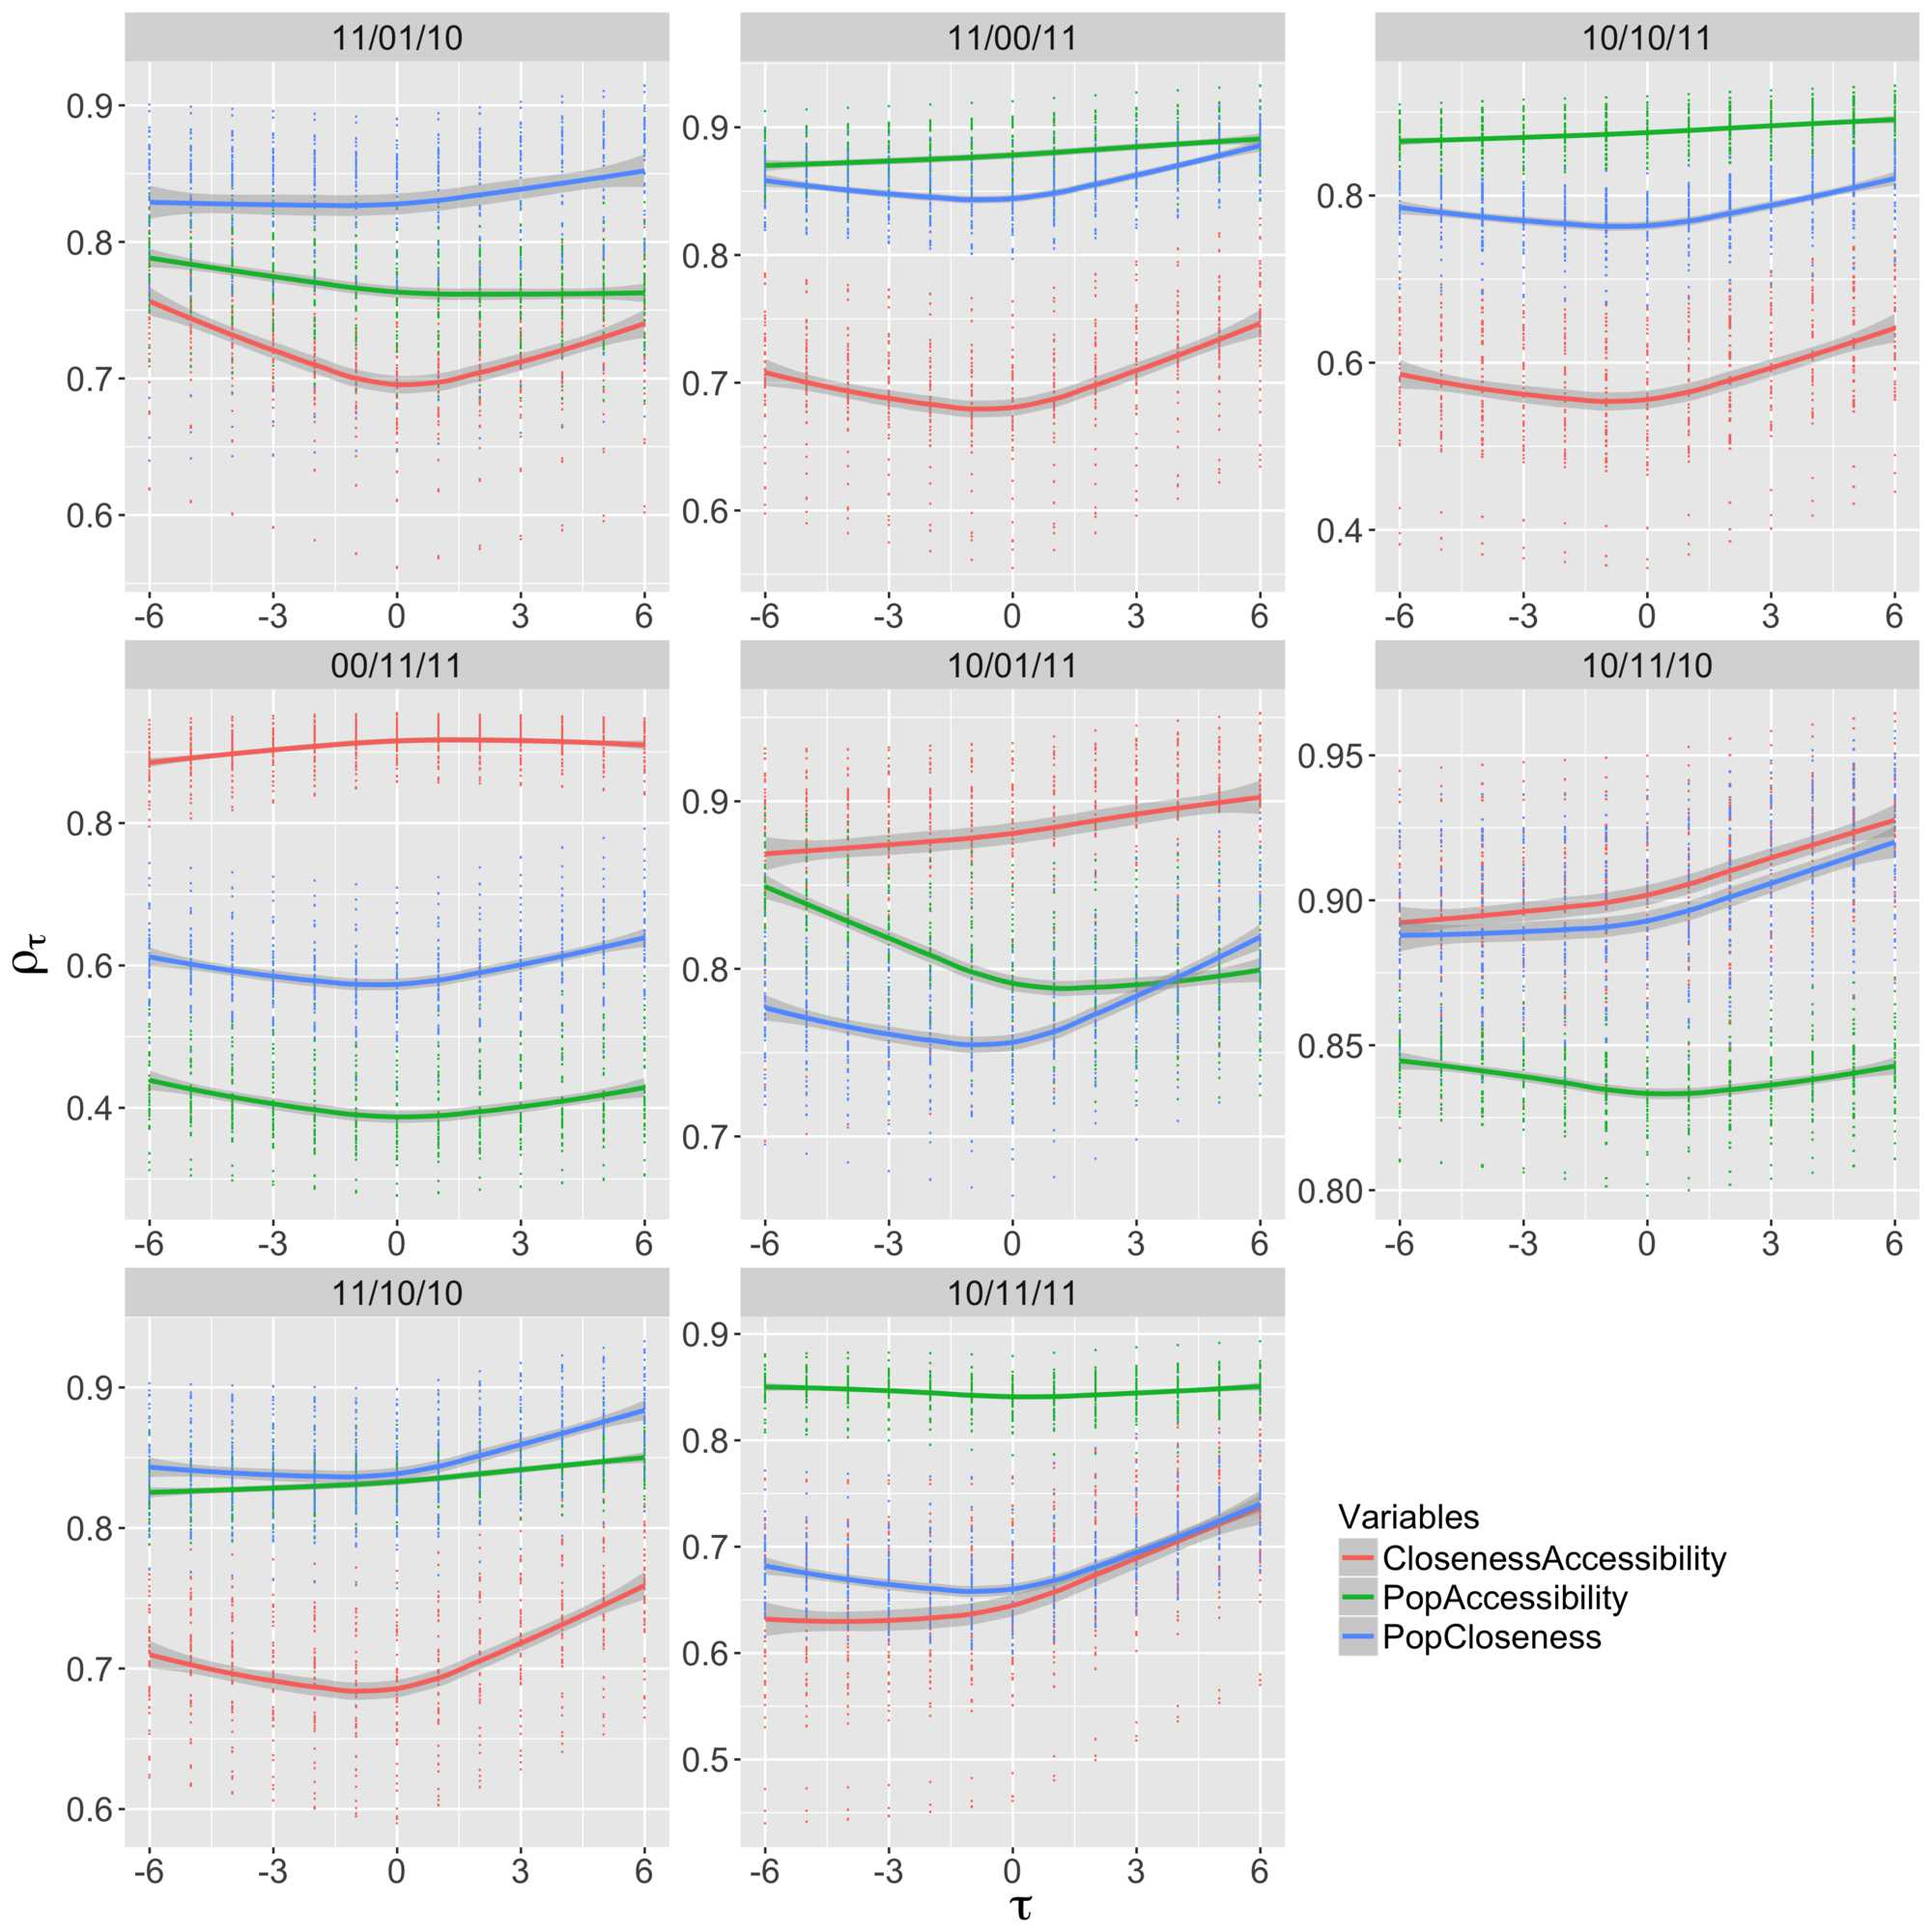
\includegraphics[width=0.39\linewidth]{figures/6-2-2-fig-macrocoevol-correlations.jpg}



\nocite{raimbault2021modeling}


\bigskip

\tiny

Raimbault, J. (2020). Indirect evidence of network effects in a system of cities. \textit{Environment and Planning B: Urban Analytics and City Science, 47}(1), 138-155.

\nocite{raimbault2020indirect}

\smallskip

Raimbault, J. (2021). Modeling the co-evolution of cities and networks. In Niel, Z., Rozenblat, C., eds. \textit{Handbook of Cities and Networks}, pp. 166-193. Edward Elgar Publishing.

\smallskip

Raimbault, J. (2022). Hierarchy and co-evolution processes in urban systems, forthcoming in Fen-Chong J., ed., \textit{Centralities and Hierarchy of Networks and Territories}, ISTE Editions. arXiv:2001.11989

\nocite{raimbault2022hierarchy}

}


\sframe{Modèles mésoscopiques de co-évolution}{

\footnotesize

%Relation entre forme et fonction (morphogenèse) comme paradigme pour modéliser la co-évolution à l'échelle mésoscopique.
%\smallskip


\justify
\textit{Modèle par réaction-diffusion et multi-modélisation de la croissance du réseau : complémentarité des heuristiques, calibration sur les formes et leurs corrélations}

\medskip

\begin{center}
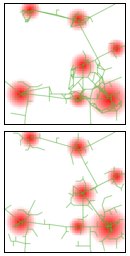
\includegraphics[width=0.29\linewidth,height=0.6\textheight]{figures/meso-nwgrowth.png}
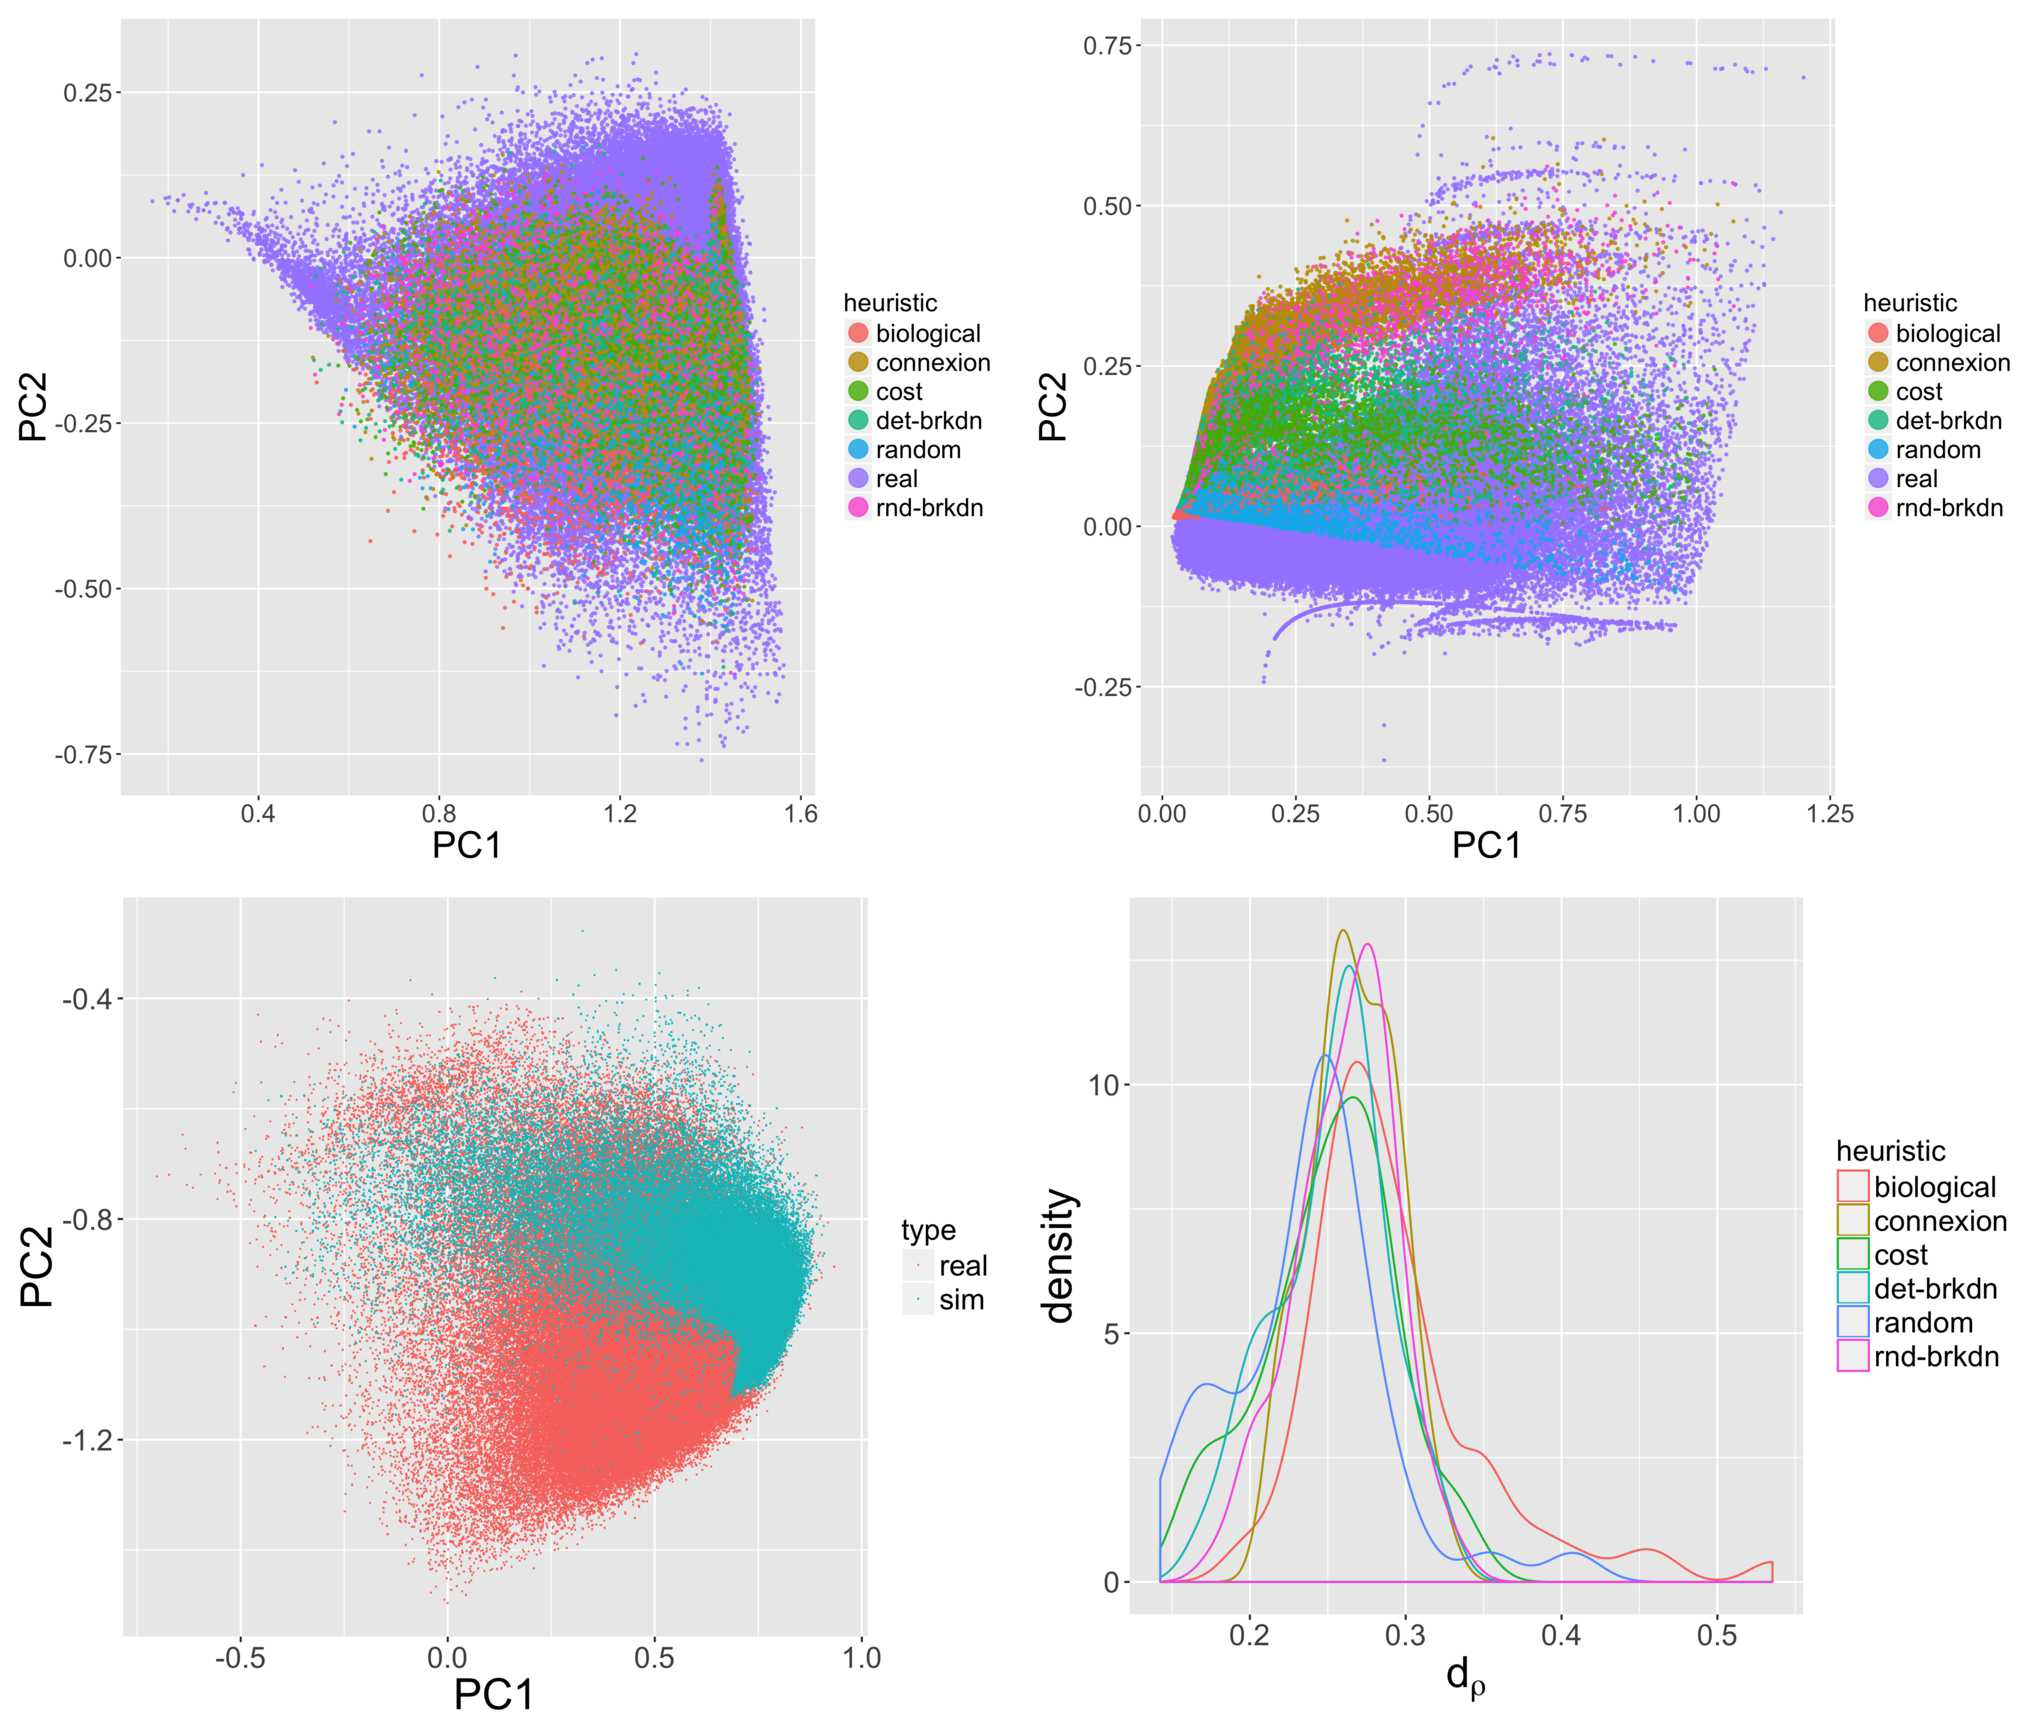
\includegraphics[width=0.69\linewidth,height=0.6\textheight]{figures/meso-calib.jpg}
\end{center}

\bigskip

\tiny

Raimbault, J. (2018). Calibration of a density-based model of urban morphogenesis. PloS one, 13(9), e0203516.

\nocite{raimbault2018calibration}

\smallskip

Raimbault, J. (2018). Multi-modeling the morphogenesis of transportation networks. In Artificial Life Conference Proceedings (pp. 382-383). MIT Press.

\nocite{raimbault2018multi}

\smallskip

Raimbault, J. (2019). An urban morphogenesis model capturing interactions between networks and territories. In The mathematics of urban morphology (pp. 383-409). Birkhäuser, Cham.

\nocite{raimbault2019urban}

}



\sframe{Co-évolution et gouvernance des transports}{

\begin{center}
	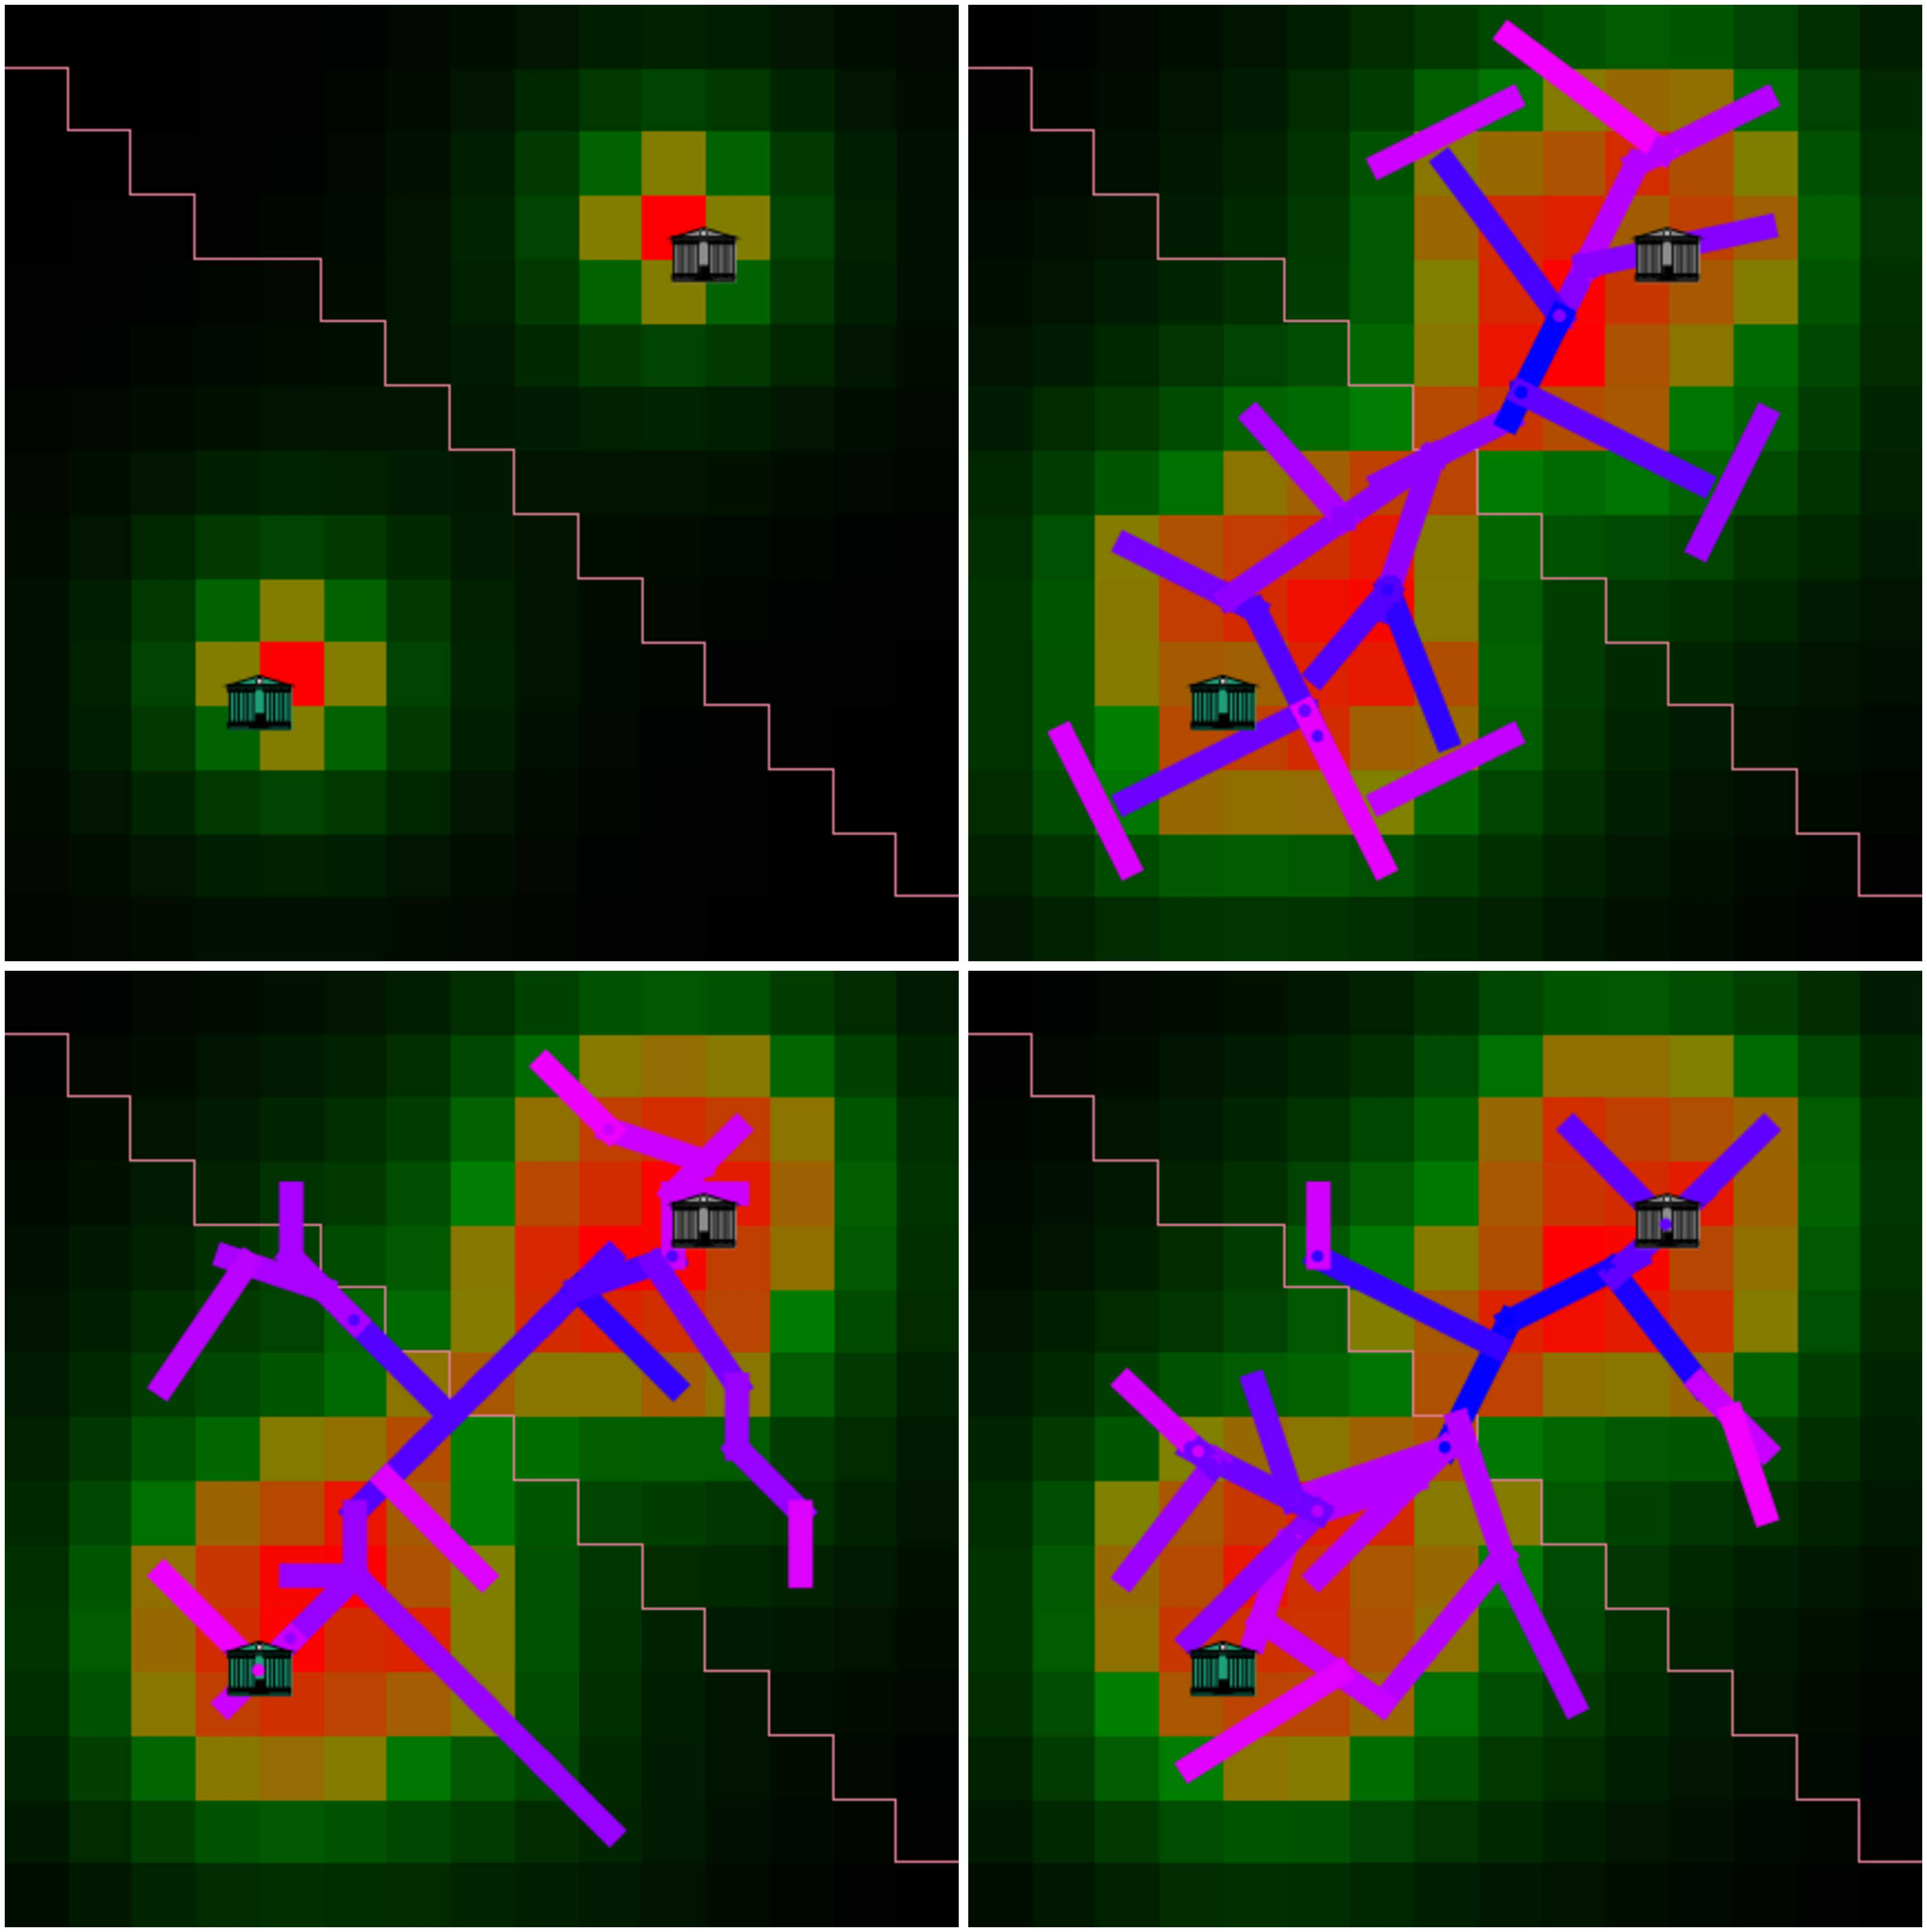
\includegraphics[width=0.5\textwidth]{figures/7-3-3-fig-lutecia-governance.jpg}
\end{center}

\textit{Simulation de l'impact des décisions d'acteurs de la gouvernance des transports}

\bigskip

\tiny

Raimbault, J., \& Le Néchet, F. (2021). Introducing endogenous transport provision in a LUTI model to explore polycentric governance systems. Journal of Transport Geography, 94, 103115.

\nocite{raimbault2021introducing}

}




\sframe{Validation des modèles: analyse de sensibilité spatiale}{

\centering

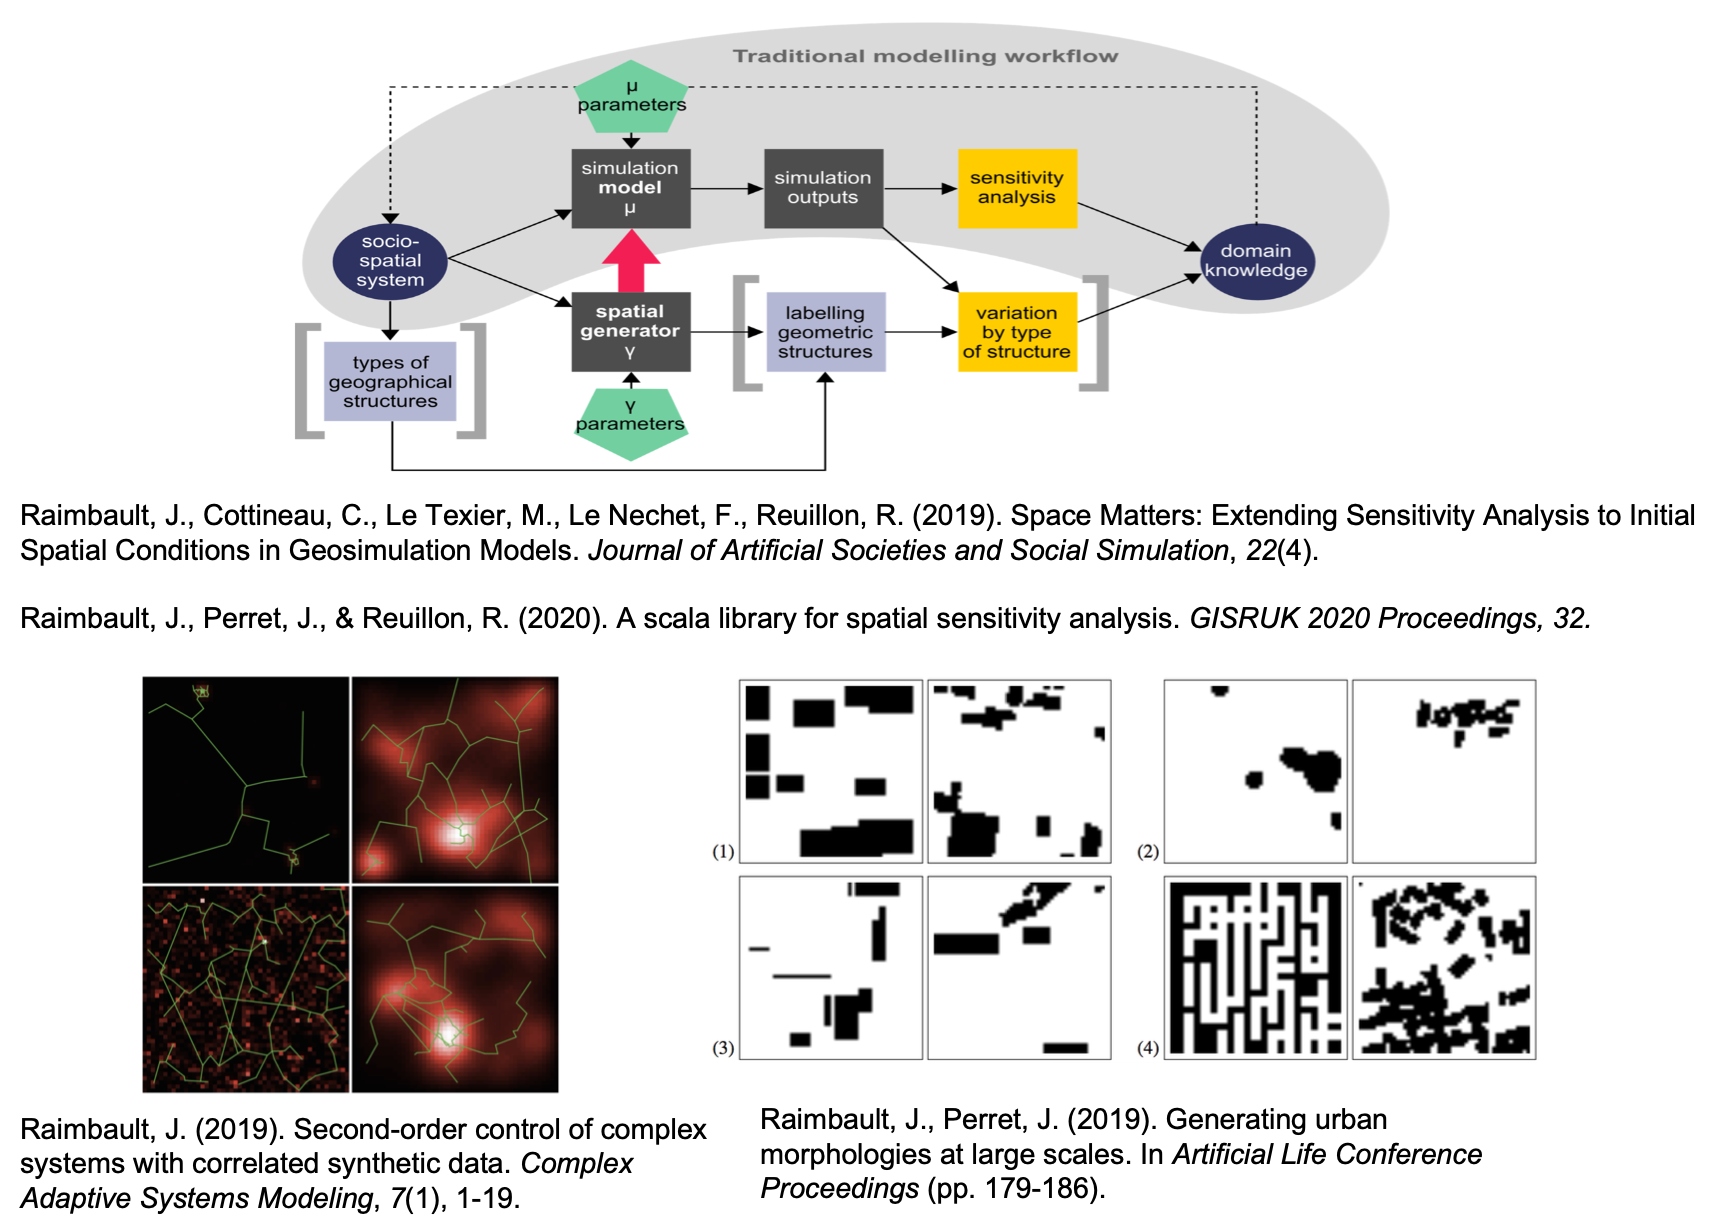
\includegraphics[width=0.95\linewidth]{figures/spatial_sa.png}

\nocite{raimbault2019second}
\nocite{raimbault2019generating}
\nocite{raimbault2019space}

}



\sframe{Propositions pour le WP3}{

%\justify

\textbf{Méthodologique : } comparaison de méthodes pour caractériser une co-évolution (inférence causale \cite{yao2021survey}, diff-in-diff \cite{lechner2011estimation}, variables instrumentales \cite{baiocchi2014instrumental}, contrôle synthétique \cite{ben2021augmented}, effets structurants \cite{bonnafous1974methodologies})

\bigskip

\textbf{Thématique : } étude empirique de la co-évolution.

$\rightarrow$ \textit{Objets ?} aménités - réseau routier ? diffusion de l'innovation ? \cite{bergeaud2017classifying}

$\rightarrow$ \textit{Echelles ? } intra-urbain / urbain ?

\bigskip

\textbf{Modélisation : } processus sous-jacents aux dynamiques urbaines et de réseau.

$\rightarrow$ \textit{Echelles ?} urbain / inter-urbain ? Multiscalaire ? (données de GeohistoricalData)


}






%%%%%%%%%%%%%%%%%%%%%
\begin{frame}[allowframebreaks]
\frametitle{References}
\bibliographystyle{apalike}
\bibliography{biblio}
\end{frame}
%%%%%%%%%%%%%%%%%%%%%%%%%%%%










\end{document}




